\textbf{Date:} May 22th 2014\\\textbf{Duration:} 10-16\\\textbf{Group
members:} Henrik, Jakob, Jesper

\subsection{Goals for today}

Come up with a way to manipulate solar panels.

\subsection{Plan:}

\begin{itemize}
\itemsep1pt\parskip0pt\parsep0pt
\item
  Make a list of requirements for turning and moving solar panels.
\item
  Brainstorm ideas for how to satisfy these.
\item
  Discuss proposals.
\item
  Decide on design of mechanism.
\end{itemize}

\subsection{List of design requirements:}

\begin{itemize}
\itemsep1pt\parskip0pt\parsep0pt
\item
  Must be able to turn a solar panel 180 degrees.
\item
  Must be able to identify working, broken, misplaced and missing solar
  panels.
\item
  Must be able to hold onto a solar panel for replacement.
\item
  Must be able to carry a solar panel past other solar panels on the
  track.
\end{itemize}

\subsection{Ideas:}

\begin{itemize}
\itemsep1pt\parskip0pt\parsep0pt
\item
  Turn a solar panel by rotating the entire vehicle.
\begin{itemize}
\item
  We have to make sure the solar panel is in the center of the vehicle,
  or it will move outside of the designated area.
\item
  No third motor is necessary, however if we want to also be able to
  move the panel around, we will need some mechanism to hold onto it.
  Even if we add some mechanism for grabbing onto the panel, we will run
  into trouble later if we need to move it around, as it will be in the
  way of other panels on the track.
\end{itemize}
\item
  Have a separate mechanism for rotating a solar panel, running on its
  own motor.
\begin{itemize}
\item
  Here we will also be able to move a panel around by turning it 90
  degrees to lock it under the vehicle. Then we can push the panel
  around, but again we will run into trouble when we need to get past
  other panels on the track.
  \end{itemize}
\item
  Lift up the solar panel, turn the entire vehicle, and put the panel
  back down.
\begin{itemize}
\item
  It will have a mechanism for holding onto a panel and lifting it from
  the track. This might be difficult to implement using only a single
  motor, but if done properly it will let us pass other panels without
  touching them. One way to do it would be to take advantage of the gap
  in the solar panels and use a thin rod to stick in the gap. The
  problem with this is that we need incredible precision in order to hit
  the target, but if we can follow the lines accurately enough, it may
  be possible.
\end{itemize}
\item
  Vehicle with a truck bed for storing defect panels; the vehicle will
  collect all the black panels so it will not have to worry about them
  later on.
\begin{itemize}
\item
  This will make it easier to bring in the replacement panels.
\item
  It will need a mechanism for lifting up the panels, perhaps we could
  implement this and the above proposal together, which, while difficult
  to implement, satisfies all the requirements.
\end{itemize}
\item
  We will have a mechanism that pushes a solar panel to the side, into a
  slot where it will be held onto. This way it will not be in the way
  when passing other solar panels and can be easily transported. To put
  the solar panel back into position on the track, we will simply put
  the mechanism in reverse, and so it only requires one motor.
\end{itemize}

We decided that the best solution will be to lift up the solar panels.
It will solve all of the requirements, and if we can implement it
properly, we will have a good shot at completing the objective. However,
the precision required is worrying, so first off we will attempt to
make a precise line follower.\\We need it to able to hit within 2 mm of
the gap. We wrote a basic line follower to test, but we immediately ran
into issues with recognizing different colors.\\
\begin{figure}[hpt]
  \centering
  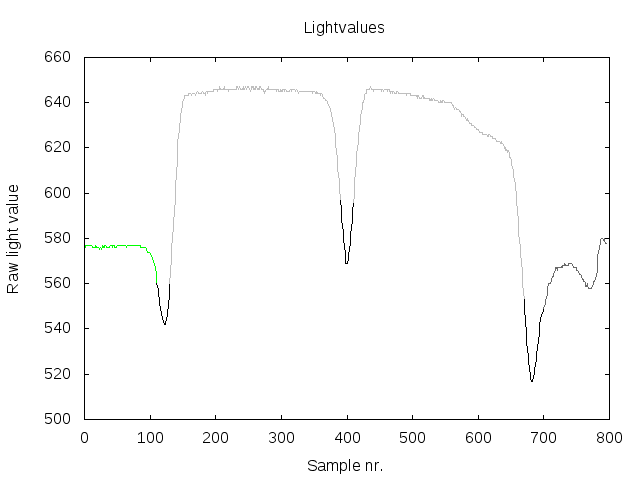
\includegraphics[scale=0.5]{../experiments/1prototype/results/gnuplot/GridAccuracy3cm_color.png}
  \caption{Light reading for a simple run from the base to the garage in a straight line (with the light sensor 3 cm above the track).}
\end{figure}
We tested the light sensor's ability to distinguish colors by letting it
start in the green starting zone, drive out across the white area,
cross a single black line, more white, and finally into the gray
storage area. As seen, green is about the same value as black, which
might cause trouble later on if we need to determine which area we are
in. One solution would be to replace it with a color sensor, but we will
return to this if it becomes necessary.

\subsection{Conclusion}

We decided on lifting solar panels and storing defect ones in addition
to the line follower. This will make the foundation for our first
prototype, and now we need to start building and testing. However, we
immediately ran into trouble when we started testing the precision of
the line follower. We will continue the testing next time, and depending
on the result, we may change strategies.
